
% ---- File-Header, Umlautpaket geladen
% \documentclass[a4paper,10pt,twocolumn,headspline]{article}
\documentclass[a4paper,10pt,headspline]{article}
% ��� f�r Mac
\usepackage[applemac]{inputenc}
%��� Universal
%\usepackage[utf8]{inputenc}
%\usepackage[ngerman]{babel}
\usepackage[pdftex]{graphicx}
\usepackage{amsmath}
\usepackage{multicol}
\usepackage{color}

% ----2011-11-04, RS: Use acronym package
%\usepackage[printonlyused]{acronym}

% ----2011-11-14, RS: Adding some colors
\usepackage{color}
\usepackage[table]{xcolor}

% ----2011-11-14, RS: Layout definition
%     I use this template for protocols.
\setlength{\textheight}{24.2cm}
\setlength{\textwidth}{17cm}
\setlength{\topmargin}{-1.6cm}
\setlength{\headheight}{0.5cm}
\setlength{\headsep}{0.8cm}
\setlength{\footskip}{0.8cm}
\setlength{\oddsidemargin}{-1.0cm}
\setlength{\evensidemargin}{-1.0cm}
\setlength{\parindent}{0cm}
\setlength{\parskip}{6pt}
\linespread{1.1}

% ----tabularx package
\usepackage{tabularx}
\usepackage[small,bf]{caption}
\usepackage{ulem}

% ----to place figures and tables within multicols
\makeatletter
\newenvironment{tablehere}
  {\def\@captype{table}}
  {}

% ----Figurehere environment
\newenvironment{figurehere}
  {\def\@captype{figure}}
  {}
\makeatother

% ----2012-03-15, RS: Custom environment
%     for script filenames
\definecolor{coldocfile}{rgb}{0.5,0,0.5}
\newcommand{\docfile}[1]{\textcolor{coldocfile}{\textbf{#1}}}
\definecolor{coldocfunc}{rgb}{0.5,0.2,0.3}
\newcommand{\docfunc}[1]{\textcolor{coldocfunc}{\textbf{#1}}}

% ----2012-03-16, RS: New command for
%     code (verbatim) and quote (quotation marks)
\definecolor{colcode}{rgb}{0.3,0.3,1.0}
\newcommand{\code}[1]{\textcolor{colcode}{\texttt{#1}}}
\newcommand{\q}[1]{``#1''}
\newcommand{\qcode}[1]{\q{\textcolor{colcode}{\texttt{#1}}}}
\newcommand{\todo}[1]{\textcolor{red}{\textbf{TODO: #1}}}

% ----2014-09-25: Update infostuff
\definecolor{colupdate}{rgb}{0.1,0.3,0.8}
\newcommand{\update}[1]{\textcolor{colupdate}{#1}}


% ----Document start
\begin{document}

% ---- Definition des Titels
\title{\vspace{0cm}Wetterturnier \\ http://wt.wetterleuchte.ch \\ \sout{Dokumentation} Infosheet}
\author{Reto Stauffer}
\date{\today}
\begin{huge}
\maketitle
\end{huge}

%\begin{center}
%Institut of Meteorologie und Geophysik
%\end{center}


\section*{Development-Environment}

Falls es jemand vergessen hat, das Zeugs ist hier:

\textbf{http://wt.wetterleuchte.ch}

\section*{Einleitende Worte}

Dies hier ist die (hoffentlich irgenwann vollst\"andige) Dokumentation
zum neuen Wetterturnier und soll dabei helfen zu verstehen, wie es
vom Aufbau her funktioniert und wie die Zusammeh\"ange sowie 
Datenbankstrukturen sind.

Marcus: ich habe f\"ur dich das Layout auch ein bisschen mehr
ans alte System angelehnt :). Achtung: da alles dynamisch ist
heisst es nicht, dass das so bleiben muss. Aber sieht irgendwie
ganz komod aus. Zumindest besser als das vorige Standard-Gr\"un-Schwarz,
aber wenn ihr Ideen habt nur zu!


\section*{Weiteres Vorgehen}

Ich bin also dran, aber so ratzfatz wird das System wohl noch nicht
fertig sein. Gerne aber gebe ich euch auch einmal einen Login und
ihr k\"onnt im Admin-Bereich rumschn\"uffeln (den Test-Login gibt 
es nicht mehr). 

Wir k\"onnten auch das Forum f\"ur Diskussionen verwenden, allerdings
finde ich es noch den falschen Zeitpunkt.
\update{Die Benutzer habe ich ebenfalls alle migriert. All jene,
die auch im htaccess file standen, sollten auch ihr altes Passwort
haben. Ihr k\"onnt dies gerne mit euerem Benutzer testen. Ihr 
seid im Moment als ``normale User'' drin, also noch kein Zugang zum
Admin-Bereich. Den m\"usste ich euch noch freischalten.} 

Irgendwann -- wenn es denn dann l\"auft auf prognose2 an der FU --
waere es cool, wenn jeder der St\"adte-Betreuer drei, vier Leute
motivieren k\"onnte, das System produktiv im Parallelbetrieb zu testen.
Dann k\"onnen wir gucken, ob alles wie erwartet funktioniert.

% -------------------------------------------------------------------
\newpage
\tableofcontents
\newpage

\setcounter{section}{0}

% -------------------------------------------------------------------
\section{Das System in wenigen Worten}

\subsection{Das Frontend: warum Wordpress?}

Ich habe mich entschieden, das gesamte System in ein Wordpress zu
integrieren. Der Grund: Wordpress bietet heute ein sehr starkes
und flexibles System zum verwalten von CMS Seiten (urspr\"unglich
als reine blogging-Software entwickelt). Es gibt so ziemlich
f\"ur Alles ein Plugin, welche meistens auch recht simpel zu 
adaptieren sind.

Dieses Framework bietet die M\"oglichkeit, alles \"uber einen
single-login zu verwalten. Das heisst: jeder Mitspieler 
erstellt einen Wordpress-Benutzer. Dieser gilt danach gleichzeitig
zum abgeben von Tips, mitplaudern im Forum und kann auch dazu
genutzt werden, gewissen Mitgliedern Admin-Rechte zuzuschreiben,
so dass diese im Backend das Wetterturnier mitverwalten k\"onnen.

\subsection{Multilingual}

Das System ist komplett bilingual. Im Wordpress m\"ussen also
Artikel oder Seiten jeweils einmal in Deutsch und einmal in
Englisch verfasstw erden - ist aber recht simpel.
Es liessen sich theoretisch auch noch weitere Sprachen hinzuf\"ugen.

\subsection{Das Wetterturnier-Plugin}

\begin{minipage}{0.19\textwidth}
   \begin{figurehere}
      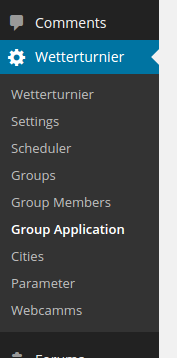
\includegraphics[width=3cm]{images/plugin.png}
   \end{figurehere}
\end{minipage}
\hfill
\begin{minipage}{0.8\textwidth}
   Das Wetterturnier im Frontend ist ebenfalls ein Wordpress-Plugin
   und vollst\"andig an Wordpress gekoppelt (also die komplette
   Benutzerverwaltung eigentlich). Das Wetterturnier kann somit
   vollst\"andig \"uber den Browser (Admin-Frontend von Wordpress)
   verwaltet werden.
   
   Genutzt wird also sowohl die User-Datenbank des Wordpress-Systems
   (\code{wp\_users}) als auch eigene Tabellen (\code{wp\_wetterturnier\_*})
   zum verwalten der Tips, Gruppen, Mitspieler, Termine, ...).
   Dieser Teil ist in \code{php}, \code{html}, \code{css}, \code{jQuery} geschrieben.
\end{minipage}
   
\subsection{Das Backend}

Im Hintergrund laufen einige Scipts, welche vom User nicht erreicht
werden k\"onnen. Massgeblich sind dies im Moment \code{Python} scripts.
W\"ahrend der Entwicklung auch diverse Scripts zum migrieren der aktuellen
Daten, welche sp\"ater nicht mehr verwendet werden.

Vorteil: mit den \code{Python}-Scripts lassen sich direkt die \code{MySQL}
Datenbanken bef\"ullen, manipulieren oder l\"oschen. Zwischen dem 
Frontend und dem Backend steht also nur die Datenbank, was das System
recht fein modular machen soll (sofern mit dies gelnugen ist :) ).

\subsection{Passwortgesch\"utzte Daten (htaccess)}

\update{Es gibt am wetterturnier-Server noch einige Maps und Forecasts,
die im Moment durch htaccess gesch\"utzt sind. Ich habe nach einigem
\"uberlegen dieses Konzept \"ubernommen. Das ``Problem'' war, dass
Wordpress eine phpass Verschl\"usselung f\"ur die Passw\"orter
verwendet, htaccess jedoch damit nicht arbeiten kann. Folgendes ist
meine L\"osung: der Benutzer wird aufgefordert, sein Passwort 
noch einmal einzugeben (obwohl er schon eingeloggt ist). Stimmt
das Passwort mit seinem Wordpress-Passwort \"uberein, so speichere
ich dieses md5-Verschl\"usselt in eine neue Tabelle und starte
am Server ein Python-Script (\code{htaccess.py}). Dieses regeneriert
das htaccess user:passwort File und der Benutzer sollte mit seinem
Wordpress login (gleicher user/pass) auch Zugriff auf diese Daten 
haben. Einziger Nachteil: \"andert er das Passwort in Wordpress, so
\"andert jenes in htaccess nicht automatisch mit, er muss da also
das alte Passwort verwenden - oder es eben nochmals kurz neu setzen.}


% -------------------------------------------------------------------
\newpage
\section{Tips abgeben, Punktevergabe, Settings}

\begin{center}
\begin{figurehere}
   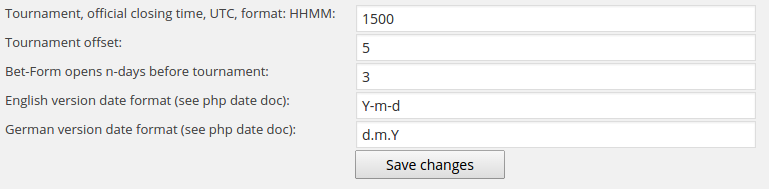
\includegraphics[width=\textwidth]{images/settings.png}
\end{figurehere}
\end{center}

Es gibt im Admin-Frontend einige Settings, die f\"ur das Tippen
wichtig sind und auch dort angepasst werden k\"onnen.

\begin{description}
   \item[official closing time] Das ist die Zeit (UTC), bis
      zu welchem die Tips abgegeben werden k\"onnen. Der Benutzer
      wird auch genau auf diese Zeit aufmerksam gemacht.
   \item[offset] Da Georg kein Henker ist, hat er gemeint, dass
      man es doch nicht so eng nehmen soll mit der Zeit. Da eine
      Zufalls-Zeit auch nicht das gelbe vom Ei ist, habe ich einen
      offset eingebaut. Das heisst in diesem Falle $5$ Minuten.
      Galgenfrist ist also \q{official closing time + offset}
      oder eben 15:05 UTC. Danach geht nix mehr.
   \item[opening] das Abgabeformular ist immer f\"ur das 
      kommende Turnier, \"offnet aber erst X Tage davor.
      So wie hier eingestellt also 3 Tage vorher - also Mittwoch
      fr\"uh um 00:00 UTC. Einstellbar aber wohl nicht so wichtig.
      Sind zwei Turniere hintereinander geplant (z.B. Freitag eins
      und Samstag eins) sollte das f\"ur Samstag am Samstag um 00:00
      ge\"offnet sein. 
\end{description}

Da gibt es vielleicht noch das eine oder andere zu tweaken, da ich
keinen offiziellen Testbetrieb habe ist es schwierig, alle
Eventualit\"aten abzufangen (dazu kommt dann die Testphase).

\begin{center}
\begin{figurehere}
   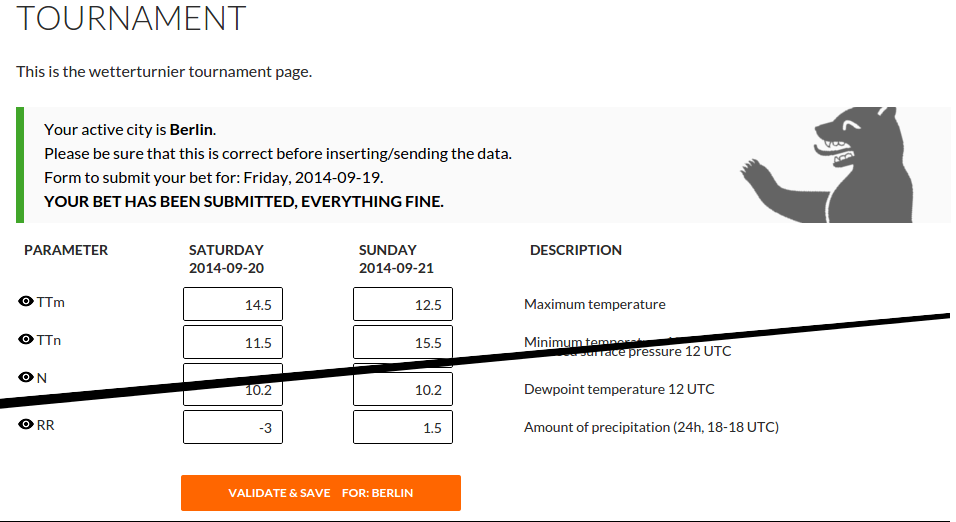
\includegraphics[width=\textwidth]{images/betform.png}
\end{figurehere}
\end{center}

\subsection{Abgabeformular}

Sobald das Turnier ge\"offnet hat -- bis zur Abgabezeit plus Galgenfrist --
k\"onnen die Benutzer ihre Tips \"uber das Abgabeformular abgeben.

\todo{Reto: ich galube, unter dem Auge wollte ich noch Hilfen anbieten. 
Oder so. Noch checken.}

\subsubsection{Validierung}

Das Abgabeformular ist jetzt auch etwas moderner. Bevor irgendwelche
Werte gespeichert werden k\"onnen, werden sie verifiziert. Werte m\"ussen
in einem gewissen Bereich sein, ansonsten werden diese nicht angenommen.
Das soll verhindern, dass irgend jemand falsche Parameter zuordnet.

\subsection{Zwischenspeichern}

Auch Neu (da mich das immer reingeritten hat): man kann nun Werte
zwischenspeichern. Das heisst: der Benutzer kann Teile aller Werte
eingeben, diese Speichern, den Arbeitsplatz verlassen und sp\"ater
weitertippen - die alten Tips bleiben bestehen.

\subsection{Finale Abgabe}

Wenn das Validierungs-Script
mit allen Werte einverstanden ist und alle Werte gesetzt wurden, wird der
Tip erst final abgegeben. Eine Warnmeldung zeigt den Status an.
Nur unvollst\"andig abgegebene Tips sind in der Datenbank gekennzeichnet (inaktiv)
und werden f\"ur das Turnier ignoriert.
Die Tips -- auch wenn bereits \q{gesendet} k\"onnen nat\"urlich noch bis
zum Ende der Abgabefrist angepasst werden.
\todo{Reto: was, wenn ein Benutzer dann einen Wert l\"oscht? Geht der
Status auch wieder auf 0 (nicht vollst\"andig)? Testen.}

\subsection{Anpassen der Tips (Admin)}

Geht noch nicht, aber die Tips sollten auch im Admin-Interface
easy angepasst und erg\"anzt werden k\"onnen. Angepasste Tips
werden markiert, so dass dies jeder sehen kann! Mehr Transparenz :).
Es steht dann z.B. bei der TTm von Hansueli: \q{Modifiziert, Reto, 19.09.2014 17:45}.
Find ich super :).

\subsection{Punktevergabe}

\update{Ich habe mich entschlossen, die Punkte ebenfalls in der
Datenbank mitzuspeichern. Dazu l\"auft im Hintergrund wieder einmal
ein \code{Python} Script, welches bei Bedarf die Punkte vergibt.
Das macht es einfacher, Statistiken zu rechen. Ebenfalls ist das
migrieren der alten Punkte so einfacher (ich migriere nun alle
Einzelpunkte aller Spieler). Zumindest arbeite ich daran :).}


% -------------------------------------------------------------------
\newpage
\section{Die Benutzerverwaltung}

\todo{Eine Entscheidung von euch, die noch gef\"allt werden muss:
wie wollt ihr die Anmeldung? Eine Variante: jeder Benutzer darf
sich registrieren, muss sich aber von einem der Administratoren
freischalten lassen. Das heisst: im Backend einfach auf \q{Approve}
klicken und schon ist der Benutzer aktiv (mit entsprechendem
Mail-Verkehr, ist Wordpress-Standard). Man kann auch zulassen,
dass sich jeder Benutzer regististrieren kann, ohne dass jemand
diesen noch akzeptieren muss.}

Ist ein Benutzer erst einmal registriert und aktiviert, kann 
dieser sofort damit anfangen, am Wetterturnier teilzunehmen
(Forum, Tips, ...). Benutzer k\"onnen im Wordpress auch
gel\"oscht werden. 
\todo{Reto: \"uberlegen was ich da mit den Tips und
Gruppenzugeh\"origkeiten mache. Droppen?}

\subsection{Migrieren der Benutzer}

Mein Plan war, alle Benutzer so zu migrieren, wie sie jetzt am 
System sind. Allerdings gibt es einige Benutzer mit speziellen
Sonderzeichen. Diese musste ich eliminieren - es gibt also
einige Benutzer, die nun einen neuen Login-Namen haben. Ich 
muss noch schauen, welche das genau sind. Das sieht im Moment
aus wie in Tabelle \ref{tab:nicename},
die Daten stammen bereits aus mitspieler.dat, sind
also alle jemals registrierten Benutzer bei wetterturnier.de.

\begin{table}
   \centering
   \begin{tabular}{ l | l }
   \hline
   Original & Neu \\
   \hline \hline
    BB\"arRS & BBarRS \\
    Bj\"orn\_Hannover & Bjorn\_Hannover \\
    Bj\"orn\_Westerwald & Bjorn\_Westerwald \\
    D\"onerbude & Donerbude \\
    D\"usentrieb & Dusentrieb \\
    DWAB/Lukas\_M\"uller & DWAB/Lukas\_Muller \\
    Eisb\"ar & Eisbar \\
    f\"ohn & fohn \\
    F\"ohni & Fohni \\
    F\"ost & Fost \\
    Gro{\ss}OBmeister\_R & GroOBmeister\_R \\
    H\"ansch & Hansch \\
    J\"urgens & Jurgens \\
    Kn\"ofel & Knofel \\
    Lukas\_S\"udharz & Lukas\_Sudharz \\
    MeteoSchweiz/Z\"urich & MeteoSchweiz/Zurich \\
    Schneeh\"auschen & Schneehauschen \\
    Tanzb\"ar & Tanzbar \\
    Tr\"opfchen & Tropfchen \\
    V\"aterchen\_Frost & Vaterchen\_Frost \\
    Windm\"uller & Windmuller \\
   \hline
   \end{tabular}
   \caption{Liste der manipulierten Benutzernamen. 
      Stammt bereits aus mitspieler.dat.}
   \label{tab:nicename}
\end{table}

% -------------------------------------------------------------------
\newpage
\section{Gruppenverwaltung}
Es k\"onnen so viele Gruppen erstellt werden, wie notwendig sind.
Gruppen starten immer Leer, jeder Benutzer muss dann manuell
hinzugef\"ugt werden.

\todo{WAV2: ich habe mir \"uberlegt noch ein kleines \code{Python}
script zu schreiben, mit welchem gr\"ossere Gruppen mit einer
Liste an Spielern direkt erstellt werden k\"onnten. Da Georg
ja immer mal wieder eine WAV-2-Gruppe er\"offnet. Oder der
Tutor soll das von Hand machen, geht auch.}

\subsection{Mitglieder in Gruppen}

\begin{minipage}{0.34\textwidth}
   \begin{figurehere}
      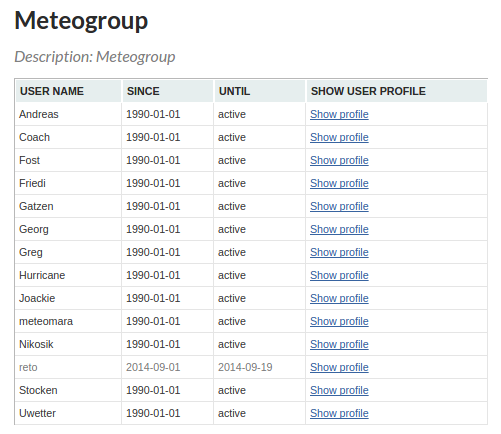
\includegraphics[width=\textwidth]{images/agroup.png}
   \end{figurehere}
\end{minipage}
\hfill
\begin{minipage}{0.65\textwidth}
   Jeder Mitspieler kann in beliebig vielen Gruppen sein, allerdings
   jeweils nur einmal (irgendwie logisch). Das System ist so aufgebaut,
   dass Benutzer beim verlassen einer Gruppe auf \q{inaktiv} gesetzt werden,
   diese Information aber nicht verloren geht. Will er in Zukunft wieder
   in dieselbe Gruppe, so wird ein neuer Eintrag erstellt - ein Benutzer
   kann also z.B. jedes zweite Jahr in einer Gruppe sein, das System sollte
   das kapieren. \todo{Reto noch klar testen, output am Frontend noch
   kontrollieren (inaktiv, von bis, aktiv, von bis).}
\end{minipage}

\subsection{Gruppenverwaltung: kann auch der User}

\begin{minipage}{0.34\textwidth}
   \begin{figurehere}
      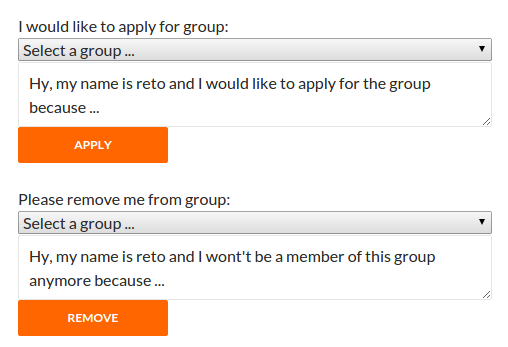
\includegraphics[width=\textwidth]{images/apply.png}
   \end{figurehere}
\end{minipage}
\hfill
\begin{minipage}{0.65\textwidth}
   Ist ein Benutzer eingeloggt, so kann er selbst auch einfluss
   auf die Gruppenzuteilung nehmen. Damit kein Wildwuchs entsteht,
   kann er sich allerdings nur \q{bewerben} bzw. auf sich aufmerksam machen.
   Auf der \q{GRUPPEN}-Seite des Wetterturniers hat er sowohl die m\"oglichkeit
   sich (mit einer Bemerkung) f\"ur eine Gruppe vorzuschlagen, andererseits
   kann er sich melden, wenn er aus einer Gruppe austreten will.
   
   Im Admin-Frontend gibt es eine Liste, in der diese Antr\"age aufgelistet
   sind. Ein Administrator kann diese Anfragen dann entweder ablehnen
   oder aber annehmen und den Benutzer so in eine Gruppe aufnehmen oder
   ihn aus der Gruppe werfen.
   
   \todo{Reto: offene applications und direkt den Benutzer in die Gruppe
   einf\"ugen koennte noch zu Konflikten f\"uhren. Hier noch \"uberpr\"ufen,
   ob noch ein Antrag offen ist und diesen updaten.}
\end{minipage}

\subsection{Gruppen-Tips}

Im Backend-Bereich gibt es ein \code{Python} script, das f\"ur alle
aktiven Gruppen die Mitteltips berechnet. Dieses Script kann
mehrfach gestartet werden, mein Vorschlag w\"are alle 15min.
So laufen auch im nachhinein noch ge\"anderte Tips direkt
in die Mitteltips ein.



% -------------------------------------------------------------------
\newpage
\section{Turnierst\"adte, Turnierpl\"ane und Parameter}

\subsection{Turnierplan, Scheduler}

\begin{minipage}{0.49\textwidth}
   \begin{figurehere}
      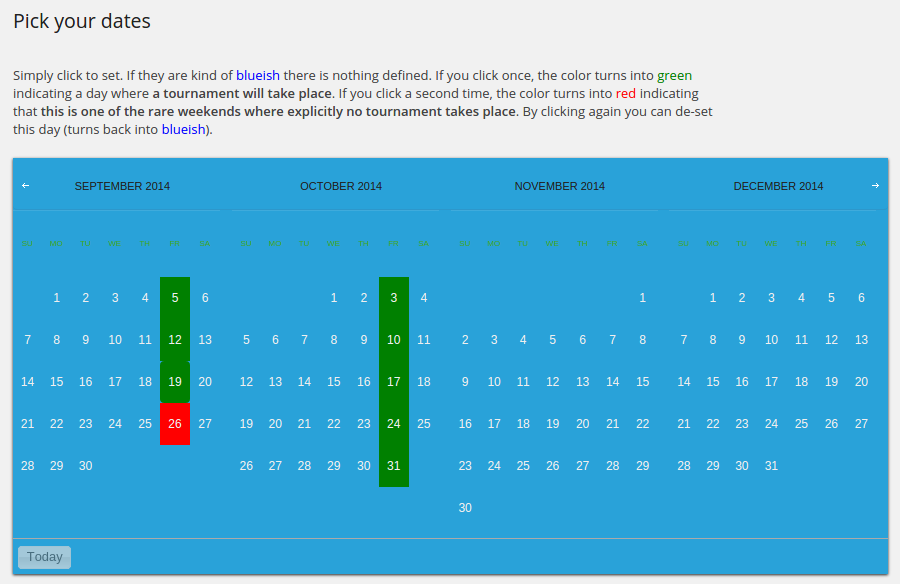
\includegraphics[width=\textwidth]{images/scheduler.png}
   \end{figurehere}
\end{minipage}
\hfill
\begin{minipage}{0.50\textwidth}
   Achtung: ich habe KEINE defaults gesetzt. Das heisst: jedes
   Turnierwochenende muss noch definiert werden. Es gibt im Backend
   einen kleinen Kalender - einmal draufklicken aktiviert den Tag als
   Turniertag, ein weiteres mal als \q{kein Turnier} (f\"ur die
   Spezialtage \"uber Weihnachten z.B.) und ein letzter dritter
   klick stellt den Tag wieder auf \q{neutral}. Da finden auch keine
   Turniere statt, sie werden aber nicht ausgewiesen.
   
   ACHTUNG: es k\"onnen auch Montage, Samstage und Dienstage als
   Turniertage definiert werden - im Prinzip. Dem System ist dies
   egal, auch wenn es wohl auch in der Zukunft ausschliesslich 
   der Freitag bleiben wird (?).
   
   PS: das Augenkrebs-Blau ist anpassbar, war mir aber noch zu wenig wichtig bis jetzt :).
\end{minipage}

\begin{minipage}{0.65\textwidth}
   Ein eigenes Turnierplan-Widget zeigt dem Benutzer auf der
   Webseite auch immer den aktuellen Stand der geplanten
   Turniere an.
   \todo{Reto noch status-ID checken}
\end{minipage}
\hfill
\begin{minipage}{0.34\textwidth}
   \begin{figurehere}
      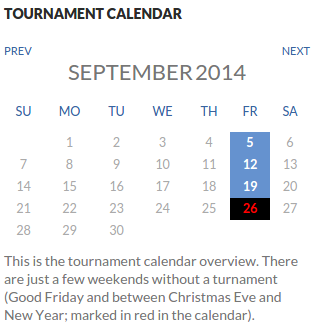
\includegraphics[width=\textwidth]{images/schedulerwidget.png}
   \end{figurehere}
\end{minipage}

\subsection{Die Turnierst\"adte}

Auch die St\"adte sind dynamisch definierbar. Man k\"onnte
das Wetterturnier also St\"adtetechnisch im Backend einschr\"anken
oder es aber erweitern. Da h\"angen dann nat\"urlich noch ein, zwei
Dinge dran (z.B. woher die Beobachtungen kommen), aber es l\"asst
sich problemlos eine weitere Stad hinzuf\"ugen.

\subsection{Parameter}

Auch Parameter lassen sich im Adminberech erweitern. Auch hier gilt:
nat\"urlich m\"ussten dann noch die automatischen Scripts (z.B. Petrus)
etc angepasst werden. Das Frontend passt sich aber automatisch an, sobald
ein neuer Parameter mit auf der Liste ist.
Ready for the future :).


% -------------------------------------------------------------------
\section{Automatische Spieler}

Ich habe schon einen Petrus gebastelt, der sollte auch schon
funktionieren. Mitteltips der Gruppen basieren auf demselben Script.
Muss man nat\"urlich noch testen, aber der war nicht so schwierig.

Bei Moses habe ich mehr Probleme bzw. brauche ich da noch Input.
Ich habe die Parameter, also die Gewichtungen, frage mich allerdings:
was passiert, wenn einer der Koeffizienten-Kollegen nicht mitspielt?
Und wo kommen die Koeffizienten her? Rechnet diese Klaus oder werden
die irgendwie irgendwo am System berechnet? Dann m\"usste man
dieses Script noch \"ubernehmen.

Bei der Persistenz muss ich noch warten bis ich die Beobachtungen
im System habe.


% -------------------------------------------------------------------
\section{Beobachtungsdaten}

Da m\"ochte ich das System \"ubernehmen, mit welchem wir Innsbruck
abgel\"osst haben bzw. abl\"osen. Da muss ich aber unseren
Informatiker noch nett bitten - und der baut gerade ein Haus und
ist derzeit wenig da. Mal gucken.


\section*{Ende ...}

Dieses Dokument ist nur eine Art Statusbericht und Todo-Liste f\"ur
mich. Feedback nat\"urlich willkommen :). Gibt aber noch das eine
oder andere zu tun.

Greez,
Reto


% -------------------------------------------------------------------
% -------------------------------------------------------------------
% -------------------------------------------------------------------
% -------------------------------------------------------------------
\newpage
\section{Database Design}

\begin{figurehere}
   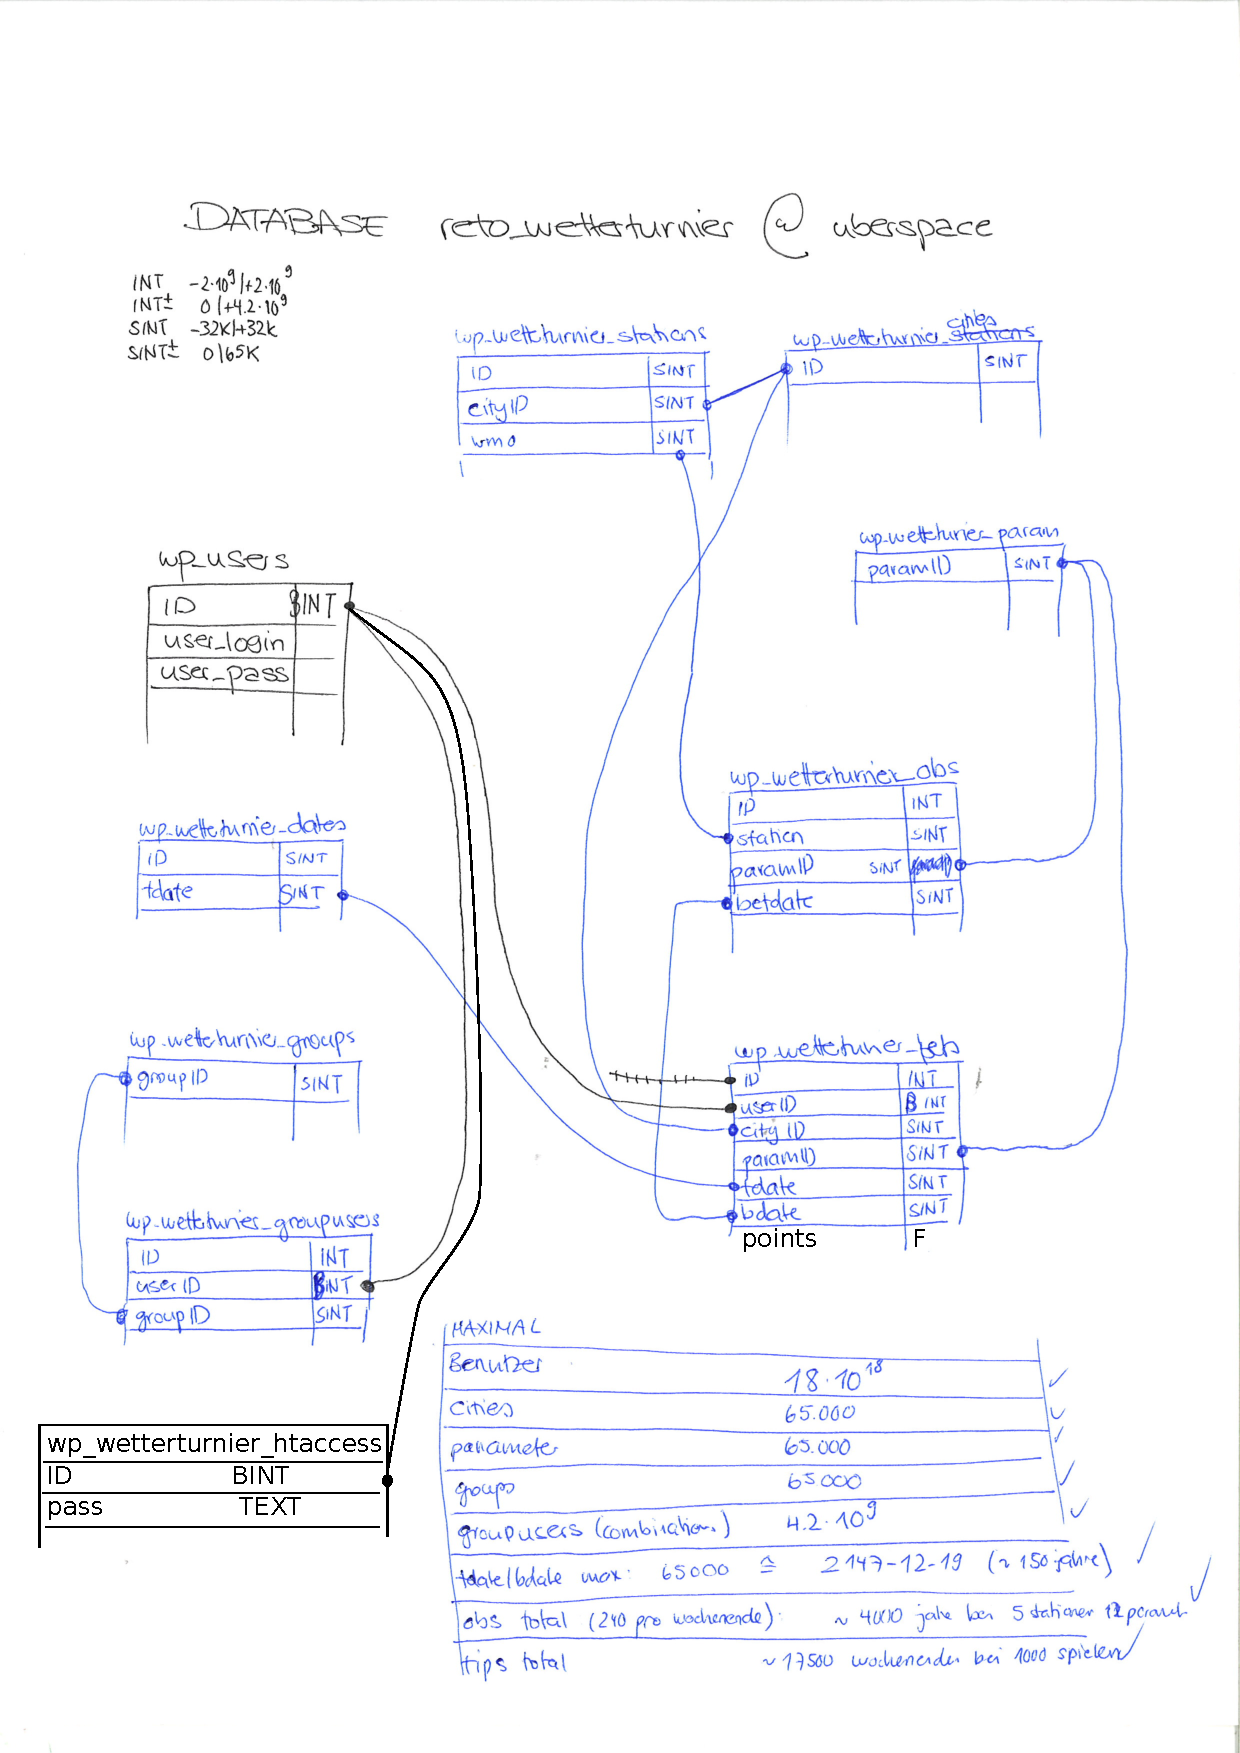
\includegraphics[height=\textheight]{scheme}
\end{figurehere}

Ich habe die Indizes noch abgeglichen und hochgerechnet. Die
auto-increments sollten f\"ur die n\"achsten paar Jahrzehnte
ausreichend sein, selbst f\"ur intensive Nutzung.
Der BIG INTEGER f\"ur die Benutzer-ID kommt vom Wordpress.
Um damit nicht in Konflikt zu kommen habe ich diesen - wenn
auch -- \"ubertrieben -- \"ubernommen.

\begin{tablehere}
   \centering
   \begin{tabular}{l|l|c|c|l}
      \hline
      Was & Typ & Limits & Pro Tag & Erwartet/Hochrechnung \\
      \hline \hline
      Benutzer (userID)     & BIGINT us  & $18e18$ & ---     & $1e3$ \\
      St\"adte (cityID)     & SINT us    & $65e3$  & ---     & ---   \\
      Parameter (paramID)   & SINT us    & $65e3$  & ---     & ---   \\
      Groups (groupID)      & SINT us    & $65e3$  & ---     & $1e2$ \\
      GroupUsers            & INT us     & $4.2e9$ & ---     & $1e3$ \\
      Tournament-/Betdates  & SINT us    & $65e3$  & $+1$    & $65e7=$ 19. Dez. 2147 \\
      Beobachtungen         & INT us     & $4.2e9$ & $250$   & $=46000$ Jahre \\
      Spielertips           & INT us     & $4.2e9$ & $2.5e4$ & $=460$ Jahre \\
      \hline
   \end{tabular}
   \caption{Hochrechnung ob die Feldtypen passen. Beobachtungen und Tips
   sind so ausgelegt, dass sie selbst bei 1000 Spielern und einem t\"aglichen
   Tipspiel die n\"achsten Jahrzehnte locker ausreichen sollten.}
\end{tablehere}

%\newpage
%\phantomsection
%\section*{Used acronyms}
%\begin{acronym}[YTM]
%  \acro{POLR}{proportional ordered logistic regression}
%\end{acronym}

\end{document}
